%\documentclass[a4paper,12pt]{book}
\documentclass[oldfontcommands]{memoir}
\renewcommand{\thefootnote}{\fnsymbol{footnote}}

%\usepackage{fourier} % or what ever
\usepackage[scaled=.92]{helvet}%. Sans serif - Helvetica
\usepackage{color,calc}
\newsavebox{\ChpNumBox}
\definecolor{ChapBlue}{rgb}{0.45,0.05,0.35}
%\definecolor{ChapBlue}{rgb}{0.00,0.65,0.65}
\makeatletter
\newcommand*{\thickhrulefill}{%
  \leavevmode\leaders\hrule height 1\p@ \hfill \kern \z@}
\newcommand*\BuildChpNum[2]{%
  \begin{tabular}[t]{@{}c@{}}
    \makebox[0pt][c]{#1\strut} \\[.5ex]
    \colorbox{ChapBlue}{%
      \rule[-10em]{0pt}{0pt}%
      \rule{1ex}{0pt}\color{white}#2\strut
%\rule{1ex}{0pt}\color{black}#2\strut
      \rule{1ex}{0pt}}%
  \end{tabular}}
\makechapterstyle{BlueBox}{%
  \renewcommand{\chapnamefont}{\large\scshape}
  \renewcommand{\chapnumfont}{\Huge\bfseries}
  \renewcommand{\chaptitlefont}{\raggedright\Huge\bfseries}
  \setlength{\beforechapskip}{20pt}
  \setlength{\midchapskip}{26pt}
  \setlength{\afterchapskip}{40pt}
  \renewcommand{\printchaptername}{}
  \renewcommand{\chapternamenum}{}
  \renewcommand{\printchapternum}{%
    \sbox{\ChpNumBox}{%
      \BuildChpNum{\chapnamefont\@chapapp}%
      {\chapnumfont\thechapter}}}
  \renewcommand{\printchapternonum}{%
    \sbox{\ChpNumBox}{%
      \BuildChpNum{\chapnamefont\vphantom{\@chapapp}}%
      {\chapnumfont\hphantom{\thechapter}}}}
  \renewcommand{\afterchapternum}{}
  \renewcommand{\printchaptertitle}[1]{%                                           
    \usebox{\ChpNumBox}\hfill
    \parbox[t]{\hsize-\wd\ChpNumBox-1em}{%
      \vspace{\midchapskip}%
      \thickhrulefill\par
      \chaptitlefont ##1\par}}%
}
\chapterstyle{BlueBox}

\usepackage[utf8x]{inputenc}
\usepackage[T1]{fontenc}
\usepackage{memhfixc}
\usepackage{hyperref}
\usepackage{url}
\usepackage{listings}
\usepackage{geometry}
\usepackage[labelfont={bf}, margin=1cm]{caption}
\usepackage{textcomp}
\usepackage{upquote}
\usepackage{multicol}
\usepackage{lscape}
\usepackage{listings}
%\usepackage{ucs}
%\usepackage{footmisc}
\usepackage[super,biblabel]{cite}

\makeatletter
\renewcommand\@biblabel[1]{#1.}
\makeatother


%\usepackage[dvipsnames]{color}

\let\footruleskip\relax % for compatibility of memoir and fancyhdr
\let\rm\rmfamily 
\usepackage{fancyhdr} 
\pagestyle{fancy}
\usepackage{arabtex}
%\usepackage{alqalam}
\usepackage{fancyvrb}
\usepackage{color}

\newcommand\at{@}
\newcommand\lb{[}
\newcommand\rb{]}
\newcommand\PYbg[1]{\textcolor[rgb]{0.00,0.50,0.00}{\textbf{#1}}}
\newcommand\PYbf[1]{\textcolor[rgb]{0.73,0.40,0.53}{\textbf{#1}}}
\newcommand\PYbe[1]{\textcolor[rgb]{0.40,0.40,0.40}{#1}}
\newcommand\PYbd[1]{\textcolor[rgb]{0.73,0.13,0.13}{#1}}
\newcommand\PYbc[1]{\textcolor[rgb]{0.00,0.50,0.00}{\textbf{#1}}}
\newcommand\PYbb[1]{\textcolor[rgb]{0.40,0.40,0.40}{#1}}
\newcommand\PYba[1]{\textcolor[rgb]{0.00,0.00,0.50}{\textbf{#1}}}
\newcommand\PYaJ[1]{\textcolor[rgb]{0.73,0.13,0.13}{#1}}
\newcommand\PYaK[1]{\textcolor[rgb]{0.00,0.00,1.00}{#1}}
\newcommand\PYaH[1]{\fcolorbox[rgb]{1.00,0.00,0.00}{1,1,1}{#1}}
\newcommand\PYaI[1]{\textcolor[rgb]{0.69,0.00,0.25}{#1}}
\newcommand\PYaN[1]{\textcolor[rgb]{0.00,0.00,1.00}{\textbf{#1}}}
\newcommand\PYaO[1]{\textcolor[rgb]{0.00,0.00,0.50}{\textbf{#1}}}
\newcommand\PYaL[1]{\textcolor[rgb]{0.73,0.73,0.73}{#1}}
\newcommand\PYaM[1]{\textcolor[rgb]{0.74,0.48,0.00}{#1}}
\newcommand\PYaB[1]{\textcolor[rgb]{0.00,0.25,0.82}{#1}}
\newcommand\PYaC[1]{\textcolor[rgb]{0.67,0.13,1.00}{#1}}
\newcommand\PYaA[1]{\textcolor[rgb]{0.00,0.50,0.00}{#1}}
\newcommand\PYaF[1]{\textcolor[rgb]{1.00,0.00,0.00}{#1}}
\newcommand\PYaG[1]{\textcolor[rgb]{0.10,0.09,0.49}{#1}}
\newcommand\PYaD[1]{\textcolor[rgb]{0.25,0.50,0.50}{\textit{#1}}}
\newcommand\PYaE[1]{\textcolor[rgb]{0.63,0.00,0.00}{#1}}
\newcommand\PYaZ[1]{\textcolor[rgb]{0.00,0.50,0.00}{\textbf{#1}}}
\newcommand\PYaX[1]{\textcolor[rgb]{0.00,0.50,0.00}{#1}}
\newcommand\PYaY[1]{\textcolor[rgb]{0.73,0.13,0.13}{#1}}
\newcommand\PYaR[1]{\textcolor[rgb]{0.10,0.09,0.49}{#1}}
\newcommand\PYaS[1]{\textcolor[rgb]{0.25,0.50,0.50}{\textit{#1}}}
\newcommand\PYaP[1]{\textcolor[rgb]{0.49,0.56,0.16}{#1}}
\newcommand\PYaQ[1]{\textcolor[rgb]{0.40,0.40,0.40}{#1}}
\newcommand\PYaV[1]{\textcolor[rgb]{0.00,0.00,1.00}{\textbf{#1}}}
\newcommand\PYaW[1]{\textcolor[rgb]{0.73,0.13,0.13}{#1}}
\newcommand\PYaT[1]{\textcolor[rgb]{0.50,0.00,0.50}{\textbf{#1}}}
\newcommand\PYaU[1]{\textcolor[rgb]{0.82,0.25,0.23}{\textbf{#1}}}
\newcommand\PYaj[1]{\textcolor[rgb]{0.00,0.50,0.00}{#1}}
\newcommand\PYak[1]{\textcolor[rgb]{0.73,0.40,0.53}{#1}}
\newcommand\PYah[1]{\textcolor[rgb]{0.63,0.63,0.00}{#1}}
\newcommand\PYai[1]{\textcolor[rgb]{0.10,0.09,0.49}{#1}}
\newcommand\PYan[1]{\textcolor[rgb]{0.67,0.13,1.00}{\textbf{#1}}}
\newcommand\PYao[1]{\textcolor[rgb]{0.73,0.40,0.13}{\textbf{#1}}}
\newcommand\PYal[1]{\textcolor[rgb]{0.25,0.50,0.50}{\textit{#1}}}
\newcommand\PYam[1]{\textbf{#1}}
\newcommand\PYab[1]{\textit{#1}}
\newcommand\PYac[1]{\textcolor[rgb]{0.73,0.13,0.13}{#1}}
\newcommand\PYaa[1]{\textcolor[rgb]{0.50,0.50,0.50}{#1}}
\newcommand\PYaf[1]{\textcolor[rgb]{0.25,0.50,0.50}{\textit{#1}}}
\newcommand\PYag[1]{\textcolor[rgb]{0.40,0.40,0.40}{#1}}
\newcommand\PYad[1]{\textcolor[rgb]{0.73,0.13,0.13}{#1}}
\newcommand\PYae[1]{\textcolor[rgb]{0.40,0.40,0.40}{#1}}
\newcommand\PYaz[1]{\textcolor[rgb]{0.00,0.63,0.00}{#1}}
\newcommand\PYax[1]{\textcolor[rgb]{0.60,0.60,0.60}{\textbf{#1}}}
\newcommand\PYay[1]{\textcolor[rgb]{0.00,0.50,0.00}{\textbf{#1}}}
\newcommand\PYar[1]{\textcolor[rgb]{0.10,0.09,0.49}{#1}}
\newcommand\PYas[1]{\textcolor[rgb]{0.73,0.13,0.13}{\textit{#1}}}
\newcommand\PYap[1]{\textcolor[rgb]{0.00,0.50,0.00}{#1}}
\newcommand\PYaq[1]{\textcolor[rgb]{0.53,0.00,0.00}{#1}}
\newcommand\PYav[1]{\textcolor[rgb]{0.00,0.50,0.00}{\textbf{#1}}}
\newcommand\PYaw[1]{\textcolor[rgb]{0.40,0.40,0.40}{#1}}
\newcommand\PYat[1]{\textcolor[rgb]{0.10,0.09,0.49}{#1}}
\newcommand\PYau[1]{\textcolor[rgb]{0.40,0.40,0.40}{#1}}
\usepackage{xcolor}
\usepackage{graphicx}

\usepackage[bahasam]{babel}
\renewcommand{\figurename}{Rajah}

\usepackage{nomencl}
\makenomenclature

\usepackage{makeidx}
\makeindex
\lstset{basicstyle=\ttfamily,frame=shadowbox}

%\chapterstyle{bianchi}

%\fancyhead[LE,RO]{\thepage}
\fancyhead[LO]{\bfseries\leftmark}
%\fancyhead[RE]{\thetitle}
\fancyhead[LE,RO]{\bfseries\thetitle}

\lstset{upquote,columns=fullflexible}

\begin{document}
\renewcommand{\figurename}{Rajah}
\renewcommand{\listfigurename}{Senarai Rajah}
\renewcommand{\nomname}{Ringkasan yang Digunakan}
\renewcommand{\bibname}{Rujukan}
\newcommand{\latex}{\LaTeX}


\title{Pengenalan kepada \LaTeX}
\author{Muhammad Najmi bin Ahmad Zabidi}
\date{}
\frontmatter
\tableofcontents
\listoffigures
\chapter{Kata Pengantar}
Terima kasih kerana memiliki buku yang tidak ternilai harganya ini.
Selamat membaca!

\chapter{\color{red}{PENAFIAN}}

Penulis {\color{red}{\textbf{tidak bertanggungjawab}}} di atas sebarang kerugian, kecelakaan, kehilangan harta benda dan sebagainya yang melibatkan tindakan yang akan mendiskreditkan penulis
 di atas kandungan buku kecil ini.
\mainmatter

\chapter{Pengenalan}
\section{Pengenalan}
\label{pengenalan}

\LaTeX{} merupakan satu perisian ``typesetting" yang dicipta oleh Leslie Lamport. \LaTeX{} berasal dari perisian \TeX{} yang ditulis oleh Donald Knuth, di mana Knuth tidak berpuas hati
dengan mutu font perisian pemprosesan perkataan sewaktu itu.

\subsection{Platform}
\LaTeX{} boleh digunakan, di antaranya di dalam sistem operasi berikut:

\begin{itemize}
\item Microsoft Windows (menggunakan WinEdt, LEd dan Lyx)
\item GNU/Linux (menggunakan \index{penyunting!Kile}Kile, \index{penyunting!Vim}VIM, \index{penyunting!Emacs}Emacs dan lain-lain penyunting)
\item Mac OS
\end{itemize}

%\paragraph
Pemilihan \index{penyunting|textbf} yang digunakan bergantung kepada citarasa pengguna, dan ia adalah sangat subjektif. Seperti saya sendiri, kadang-kadang saya menggunakan Kile dan kadang-kadang hanya 
menggunakan perisian ringan VIM. 

\subsection{Sokongan}
\LaTeX{} mempunyai peminat dan penyokongnya yang tersendiri, terdiri daripada khalayak yang menggunakannya secara intensif. Kebiasaannya, soalan teknikal berkaitan \LaTeX{} dibincangkan di dalam
mailing list ataupun forum-forum di Internet. 

\section{Sampel yang dihasilkan menggunakan \LaTeX}
\LaTeX{} banyak digunakan samada oleh pelajar-pelajar universiti yang menyiapkan laporan projek, tesis ataupun artikel ataupun mereka yang berkecimpung di dalam bidang penulisan.


\section{Font yang disokong oleh \LaTeX}
\label{sokongan}
\latex{} menyokong penggunaan font \index{Arab} Arab dan \index{Jawi} Jawi, selain daripada huruf Roman\footnote{memandangkan buku ini ditulis untuk pembaca berbahasa Melayu}.
Sebagai contoh untuk font Arab;\\\\


\vocalize
\arabtrue
\begin{RLtext}
\large{
al-salAm `alaykum
\setnash{al-salAm `alaykum,}
\setnashbf{al-salAm `alaykum,}
\setnastaliq{al-salAm `alaykum}
}
\end{RLtext}

\hspace{1cm}

Dan font Jawi;\\

\novocalize
\setmalay
<cUbA lIht tUlIsn inI,>
{\color{blue}\setnashbf{<cUbA lIht tUlIsn inI,>}}
{\color{red}\setnastaliq{<cUbA lIht tUlIsn inI,>}}\\\\

Selain itu, \latex{} juga boleh menggunakan pakej yang ditetapkan sendiri oleh pengguna (user-customized). 



\section{Kenapa guna \LaTeX?}
Ada beberapa sebab kenapa anda perlu mempertimbangkan untuk menggunakan \LaTeX{}, di antaranya ialah:

\begin{itemize}
\item sokongan perisian percuma, atau sekiranya anda mampu anda boleh membeli perisian komersial untuk membantu penulisan anda
\item sokongan Bib\TeX{}, satu perisian yang membantu anda untuk mengatur letak \mbox{``}citation\mbox{''} pada penulisan anda
\item susun atur nombor secara automatik, di mana anda tidak perlu risau tentang atur letak kepala dokumen anda (header)
\item diterima sebagai satu piawaian (standard) sekiranya anda ingin menghantar artikel ataupun jurnal ke mana-mana seminar antarabangsa (sekiranya dinyatakan)
\end{itemize}

\section{Mendapatkan pakej \latex}

\subsubsection{Windows}

Sekiranya anda menggunakan Microsoft Windows, anda boleh dapatkan pakej \latex{} yang terkandung secara pukal di dalam penginstal (berekstensi .exe).\\

\begin{itemize}

\item WinEdt\cite{winedt} 
\item Lyx\cite{lyx} 
\item LEd (Latex Editor) \cite{led}

\end{itemize}


\subsubsection{Linux}

Sekiranya anda menggunakan Ubuntu Linux dan menggunakan Kile\cite{kile}; \\

\begin{Verbatim}[frame=single]
apt-get install kile
\end{Verbatim}

dan semua kebergantungan(dependencies) akan diuruskan oleh pengurus pakej apt-get tersebut.
Sesetengah masalah pakej contohnya arabtex dan alqalam boleh dicari sekiranya anda menggunakan ``apt-cache search"

Contohnya, pakej arabtex terkandung di dalam texlive-lang-arab.



\chapter{Jom Belajar \LaTeX{}!}
\section{Belajar \LaTeX{} susahlah!}
\label{chap1}
\LaTeX{} mempunyai cerun \index{pembelajaran} yang tinggi pada mulanya, tetapi apabila sudah dipelajari, ia akan memudahkan anda untuk menyelesaikan tugasan anda.
Sekiranya anda bergiat di dalam bidang yang memerlukan penulisan persamaan (equation) contohnya, \LaTeX{} sangat membantu anda.

\section{Mengenali format \latex}
\label{kenal}
Sekiranya anda pernah mempelajari apa-apa bahasa aturcara yang berbentuk \emph{procedural}, anda akan dapati \latex mempunyai format yang hampir serupa, di mana
turutan arahan yang akan dilaksanakan adalah dari atas ke bawah. 

\latex{} mempunyai sintaks tersendiri, di mana pengguna hendaklah mengisytiharkan awalan dan akhiran dokumen. Ia adalah seperti berikut:\\


\begin{minipage}{\textwidth}
\begin{lstlisting}[frame=shadowbox,label={cth1-arahan}]
 \begin{document}
  ...di sini anda akan laksanakan arahan anda...
 \end{document}
\end{lstlisting}

\end{minipage}


\hspace{2cm}
 %\ref{cth1-arahan} 
Seperti yang anda lihat pada Contoh di atas, itu adalah sintaks permulaan bagi dokumen \latex{} anda.

\section{Bentuk penulisan}
Secara umum, ada tiga jenis kelas dokumen yang digunakan di dalam \latex{}, iaitu 

\begin{description}
 \item[article] untuk penulisan makalah, dihantar ke seminar akademik
\item[report] mirip seperti artikel
\item[book]untuk penulisan buku, terdapat sokongan indeks, penetapan isi kandungan secara automatik, kepala dokumen dan sebagainya
\end{description}

\subsection{Kelas article}
\emph{Article class} ialah salah satu kelas dokumen yang penting dan ringkas, di mana anda perlu menetapkan kategori article ini di kepala dokumen anda.
Lihat contoh di bawah:\\

\begin{lstlisting}[frame=shadowbox]
\documentclass{article}

\begin{document}

\end{document}
\end{lstlisting}

Pada setakat ini, anda hanya telah mengisytiharkan yang dokumen anda ialah sebuah artikel. Seterusnya, kita letakkan tajuk artikel dan nama pengarang
seperti di bawah:\\

\begin{lstlisting}[frame=shadowbox]
\documentclass{article}
\title{Artikel saya}
\author{Najmi}
\begin{document}
\maketitle
\end{document}
\end{lstlisting}

\bigskip
Dokumen ini akan menghasilkan output seperti berikut:\\

\begin{minipage}{\linewidth}
\centering
\fbox{
\includegraphics[scale=.7]{artikel-saya.png}}
\captionof{figure}{Artikel pertama}
\label{artikel}
\end{minipage}

\section{Bagaimana \latex{} menghasilkan dokumen?}

Secara asasnya \latex{} berfungsi seperti berikut:\\

\begin{Verbatim}[frame=single]
 fail asal (namafail.tex) ---> fail yang dijanakan (namafail.dvi)
\end{Verbatim}

Dalam kes ini, fail yang kita sunting sebagai kod sumber mempunyai sambungan .tex dan menghasilkan .dvi\index{dvi}\nomenclature{DVI}{Device Independent} . 
Tetapi, untuk memudahkan pembaca membaca dokumen yang kita hasilkan, muncullah \index{PDFLaTeX}PDFLaTeX, yang menghasilkan fail berasaskan Portable Document Format(\index{PDF}\nomenclature{PDF}{Portable Document Format} PDF).
Fail PDF boleh anda baca menggunakan pembaca PDF contohnya Acrobat Reader. Jadi dalam kes ini;\\

\begin{Verbatim}[frame=single]
 fail asal (namafail.tex) --(guna PDFLaTeX)--> fail yang dijanakan (namafail.pdf)
\end{Verbatim}

\section{Pakej di dalam \latex{}}
\latex{} memerlukan pengguna memasukkan pakej secara manual sebelum ia memproses arahan dari pengguna. Contoh-contoh pakej ialah:\\

\begin{minipage}{\textwidth}

\begin{center}
\begin{tabular}{|l|l|}
\hline
 graphicx&  untuk tujuan grafik \\ \hline
 lscape& untuk tujuan mengubah bentuk paparan kertas semasa menulis dokumen\\ \hline
 alqalam&  teks al-quran di dalam lateks\\\hline
\end{tabular}
\end{center}   
\end{minipage}
\bigskip

Jadi sebagai lanjutan untuk sebelum ini, ia akan menjadi seperti berikut:\\

\begin{lstlisting}[frame=shadowbox]
\documentclass{article}
\usepackage{graphicx}
\usepackage{lscape}
\usepackage{alqalam}

\title{Artikel saya}
\author{nama pengarang}
\begin{document}
\maketitle
\end{document}
\end{lstlisting}

\chapter{Format Tulisan}

\section{Pelbagai jenis format tulisan}

Default:
\begin{verse}
Pulau Pandan Jauh ke Tengah \\
Gunung Daik Bercabang Tiga\\
Hancur Badan Dikandung Tanah\\
Budi yang Baik Dikenang Juga\\
\end{verse}
\bigskip
Bold:
\textbf{\begin{quote}
Pulau Pandan Jauh ke Tengah \\
Gunung Daik Bercabang Tiga\\
Hancur Badan Dikandung Tanah\\
Budi yang Baik Dikenang Juga\\
\end{quote}}
\bigskip
Italics:
\textit
{\begin{quote}
Pulau Pandan Jauh ke Tengah \\
Gunung Daik Bercabang Tiga\\
Hancur Badan Dikandung Tanah\\
Budi yang Baik Dikenang Juga\\
\end{quote}
}
\bigskip
Untuk gaya \index{font}font selain di atas, secara asasnya kita gunakan:\\

\begin{Verbatim}[frame=single]
\textbf{teks anda di sini} % ini untuk bold
\textit{teks anda di sini} % ini untuk italics
\texttt{teks anda di sini} % ini untuk teletype 
\textrm{teks anda di sini} % ini untuk Roman
\textsf{teks anda di sini} % ini untuk serif
\textup{teks anda di sini} % ini untuk TitleCase
\textsl{teks anda di sini} % ini untuk font senget ke kanan
\textsc{teks anda di sini} % ini untuk font CAPS kecil
\textmd{teks anda di sini} % ini untuk font pertengahan, antara normal dan bold
\end{Verbatim}

Kita lihat contoh berikut untuk campuran font ini:\\

{\begin{quote}
\textsf{Pulau Pandan} \textrm{Jauh ke Tengah} \\
\textup{Gunung Daik} \textsl{Bercabang Tiga}\\
\textsc{Hancur Badan} \textmd{Dikandung Tanah}\\
\textbf{Budi yang Baik} \textit{Dikenang Juga}\\
\end{quote}
}

di mana ia sebenarnya adalah :\\

\begin{Verbatim}[frame=single]

{\begin{quote}
\textsf{Pulau Pandan} \textrm{Jauh ke Tengah} \\
\textup{Gunung Daik} \textsl{Bercabang Tiga}\\
\textsc{Hancur Badan} \textmd{Dikandung Tanah}\\
\textbf{Budi yang Baik} \textit{Dikenang Juga}\\
\end{quote}
}
\end{Verbatim}
\chapter{Membuat senarai}
\section{Bina senarai menggunakan \latex{}}
\latex{} membolehkan anda membuat \index{penyenaraian}penyenaraian \emph{bullet} dengan menggunakan arahan \mbox{{\\item}}.
Contoh output adalah seperti berikut:\\

\begin{itemize}
\item satu
\item dua
\item tiga
\end{itemize}

yang sebenarnya adalah:\\

\begin{Verbatim}[frame=single]
\begin{itemize}
\item satu
\item dua
\item tiga
\end{itemize}
\end{Verbatim}

selain itu, ada juga \emph{description} untuk membolehkan anda membuat penjelasan untuk perkara yang di\emph{bold}kan

\begin{description}
\item [satu] adalah nombor
\item [dua] adalah nombor selepas satu
\item [tiga] adalah nombor selepas tiga
\end{description}


\begin{Verbatim}[frame=single]
\begin{description}
\item [satu] adalah nombor
\item [dua] adalah nombor selepas satu
\item [tiga] adalah nombor selepas tiga
\end{description}
\end{Verbatim}



\chapter{Penulisan artikel}

\section{Artikel komputer}
Sekiranya anda terlibat di dalam penulisan artikel saintifik, ada kemungkinan di mana anda perlu memasukan kod sumber anda di dalam artikel anda. 
Kita lihat contoh kod yang ditulis menggunakan bahasa Python di bawah:
\bigskip

\begin{minipage}{\textwidth}
\begin{lstlisting}[frame=shadowbox,language=python]
print "Hello World!"
\end{lstlisting}
\captionof{figure}{Hello World ringkas tanpa warna}
\label{hello-simple}
\end{minipage} \\

Di samping itu, anda juga boleh menggunakan fungsi penyerlahan sintaks \textit{(syntax highlighting)} seperti tertera berikut:\\

\begin{minipage}{\textwidth}
\begin{Verbatim}[frame=single,commandchars=@\[\]]
@PYay[print] @PYaB["]@PYaB[Hello, World!]@PYaB["] 
\end{Verbatim}
\captionof{figure}{Hello World ringkas dengan warna}
\label{hello-colour}
\end{minipage} \\

Kita tengok contoh yang lain yang lebih panjang kodnya.

\begin{minipage}{\textwidth}
\begin{Verbatim}[frame=single,commandchars=@\[\]]
@PYbc[import] @PYaV[gettext]
gettext@PYbe[.]bindtextdomain (@PYaB[']@PYaB[piton]@PYaB['],@PYaB[']@PYaB[/usr/share/locale]@PYaB['])
gettext@PYbe[.]textdomain(@PYaB[']@PYaB[piton]@PYaB['])
_@PYbe[=] gettext@PYbe[.]gettext
@PYay[print] _(@PYaB[']@PYaB[python adalah mudah]@PYaB['])
@PYay[print] _(@PYaB[']@PYaB[semudah ini]@PYaB['])
\end{Verbatim}
\captionof{figure}{Kod lebih panjang dengan warna}
\label{piton}
\end{minipage} \\

dalam contoh \ref{hello-simple}, \ref{hello-colour} dan \ref{piton} di atas, arahan \emph{verbatim} digunakan supaya set arahan itu tidak dilaksanakan oleh sistem, 
sebaliknya dipaparkan ke dalam skrin.

\section{Artikel dengan formula matematik}
\latex{} boleh membantu anda menyiapkan kerja-kerja yang memerlukan anda memasukkan formula \index{matematik}matematik, termasuklah penulisan saintifik, kertas soalan, mahupun peberbitan lain. 



\subsection{Contoh formula matematik}

\subsubsection{\index{Punca kuasa}Punca kuasa}
Katakan anda ingin memasukkan punca kuasa dua di dalam dokumen anda.

$\sqrt{4} = 2$

dalam perkara ini, kebiasaannya sintaks yang ingin ditukar kepada formula matematik diapit dengan tanda \mbox{\$}.

Contohnya untuk menghasilkan formula tadi, kita tulis seperti berikut:\\

\begin{Verbatim}[frame=single]
 $\sqrt{4} = 2$
\end{Verbatim}

Di mana, dalam contoh di atas, oleh kerana kita ingin membuat punca kuasa dua, iaitu $\sqrt{4}$, maka kita letakkan nombor 4 di dalam kurungan tersebut \mbox{\{4\}}.
Bagaimana sekiranya punca kuasa tiga, empat, dan seterusnya?\\

$\sqrt[3]{8} = 2$\\

dihasilkan dengan;\\

\begin{Verbatim}[frame=single]
 $\sqrt[3]{8} = 2$
\end{Verbatim}

dan,\\

$\sqrt[4]{16} = 2$\\

dengan\\

\begin{Verbatim}[frame=single]
 $\sqrt[4]{16} = 2$
\end{Verbatim}


\subsubsection{Kuasa}
Untuk kuasa, maka seperti contohnya $x^y$, maka ia adalah seperti berikut:\\

\begin{Verbatim}[frame=single]
 $x^y$
\end{Verbatim}


%Pakej matematik di dalam \latex{} ialah menggunakan pakej \nomenclature{AMS}{American Mathematical Society} AMS.
%Untuk itu, apa yang perlu anda lakukan ialah meletakkan \\

%\begin{Verbatim}[frame=single]
% \include{ams}
%\end{Verbatim}

%pada kepala dokumen anda.
\chapter{Slaid persembahan}

\section{Membuat slaid \index{persembahan}persembahan dengan \latex{} beamer}
Kebiasaanya apabila kita mendengar \emph{presentation slides} maka yang terlintas di fikiran kita samada Microsoft(TM) PowerPoint ataupun OfficeOffice.org Impress.
Sebenarnya, \latex{} juga mempunyai pakej persembahannya yang dipanggil \mbox{"}beamer\mbox{"}.

Untuk pakej \index{beamer}beamer, kita perlu mengisytiharkan penggunaan pakej beamer, sama seperti sebelum ini:\\

\begin{Verbatim}[frame=single]
 \usepackage{beamer}
\end{Verbatim}

\subsection{Bingkai (\emph{frame})}
Di dalam beamer, setiap persembahan dipecahkan kepada beberapa bingkai atau di sini kita sebut sebagai frame. 
Cuba perhatikan kod berikut:


\begin{Verbatim}[frame=single]
 \begin{frame}
  
 \end{frame}
\end{Verbatim}

Dan sekarang tengok pula kod untum muka utama slaid kita:

\begin{Verbatim}[frame=single]
\documentclass[xcolor=dvipsnames,11pt]{beamer}
\usetheme{Luebeck} % ini untuk pilihan tema


\title[tutorial \LaTeX{}]{Pengenalan Kepada \LaTeX{}} 
% ini untuk tajuk di kaki slaid, pilihan saja

\author[Aiman]{Ahmad Abu Aiman }
% ini untuk tajuk di kaki slaid, plihan saja

\begin{document}
\begin{frame}

\title[Seminar \LaTeX{}, Segambut Dalam]{Pengenalan Kepada \LaTeX{}}
\author[Aiman]{Ahmad Abu Aiman }
\institute{
        Nama Institut,\\
        Malaysia\\
        }
\date{} 
% sekiranya tidak diisi dengan tarikh, tarikh 
%pada dokumen ini dikompil akan digunakan

\titlepage 
%ini untuk mengisytiharkan yang bingkai
% ini akan digunakan untuk muka depan


\begin{center}\texttt{email@email.com}\\
        \textrm{\tiny { Ditulis dengan \LaTeX{}}}
\end{center}


\end{frame}
\end{document}

\end{Verbatim}

\begin{minipage}{\textwidth}
Contoh output:
\begin{center}
\fbox{
\includegraphics{beamer.png}}
\end{center}
\end{minipage}

\chapter{Pakej Arab\TeX{} dan \emph{alqalam}}

\section{Arab\TeX{}}

Secara asasnya, sepanjang yang penulis ketahui tulisan Arab di dalam Arab\TeX{} dihasilkan menggunakan huruf-huruf Roman seperti berikut:\\

\begin{figure}[h!tb]
\begin{center}
\begin{tabular}{|c|c|c|c|c|c|c|c|c|c|c|c|c|c|}
\hline
\rule[-6pt]{0pt}{16pt}
<A> & <b> & <t> & <_t> & <j> & <.h> & <_h> &
<d> & <_d> & <r> & <z> & <s> & <^s> & <.s> \\
\hline
\verb#A# & \verb#b# & \verb#t# & \verb#_t# & \verb#j# & \verb#.h# & \verb#_h# &
\verb#d# & \verb#_d# & \verb#r# & \verb#z# & \verb#s# & \verb#^s# & \verb#.s#\\
\hline
\hline
\rule[-7pt]{0pt}{17pt}
<.d> & <.t> & <.z> & <`> & <.g> & <f> & <q> &
<k> & <l> & <m> & <n> & <h> & <w> & <y> \\
\hline
\verb#.d# & \verb#.t# & \verb#.z# & \verb#`# & \verb#.g# & \verb#f# & \verb#q# &
\verb#k# & \verb#l# & \verb#m# & \verb#n# & \verb#h# & \verb#w# & \verb#y# \\
\hline
\end{tabular}
\end{center}

Huruf asing, yang bukan Arab:\smallskip
\begin{center}
\begin{tabular}{|c|c|c|c|c|c|c|c|c|c|}
\hline
<p> & <v> & <^c> & <,c> & <^z> & <g> & <c> & <^n> & <^l> & <.r> \\
\hline
\verb#p# & \verb#v# & \verb#^c# & \verb#,c# & \verb#^z# & \verb#g# &
\verb#c# & \verb#^n# & \verb#^l# & \verb#.r# \\
\hline
\end{tabular}
\end{center}
\caption{Susunatur huruf dan bagaimana untuk anda tulis di dalam teks \ArabTeX{}\cite{paut-arab}}
\label{arab-rujuk}
\end{figure}

Jadual \ref{arab-rujuk} ini turut memaparkan bagaimana untuk anda menulis Jawi di dalam Arab\TeX{}.


\section{\emph{alqalam}}
Pakej ini membolehkan anda memasukkan teks al-quran, atau mencetak teks al-quran di dalam tulisan anda.
Kita tengok contoh kod yang dimuatkan di dalam sampel dari dokumentasi alqalam. Surah yang dipaparkan berikut merupakan sebahagian ayat dari
Surah as Sajadah, kod sumber \latex{} boleh dimuat turun di laman mirror Debian untuk alqalam. \cite{paut-kalam}.
%\lstset{inputencoding=utf8x, extendedchars=\true}
%
%\begin{Verbatim}[frame=single]
%\end{Verbatim}

%\lstinputlisting{sajda.tex}


%\begin{landscape}
%\begin{multicols}{2}
%\begin{minipage}{0.25\linewidth}
\begin{minipage}{\linewidth}
\begin{center}

%\fbox{
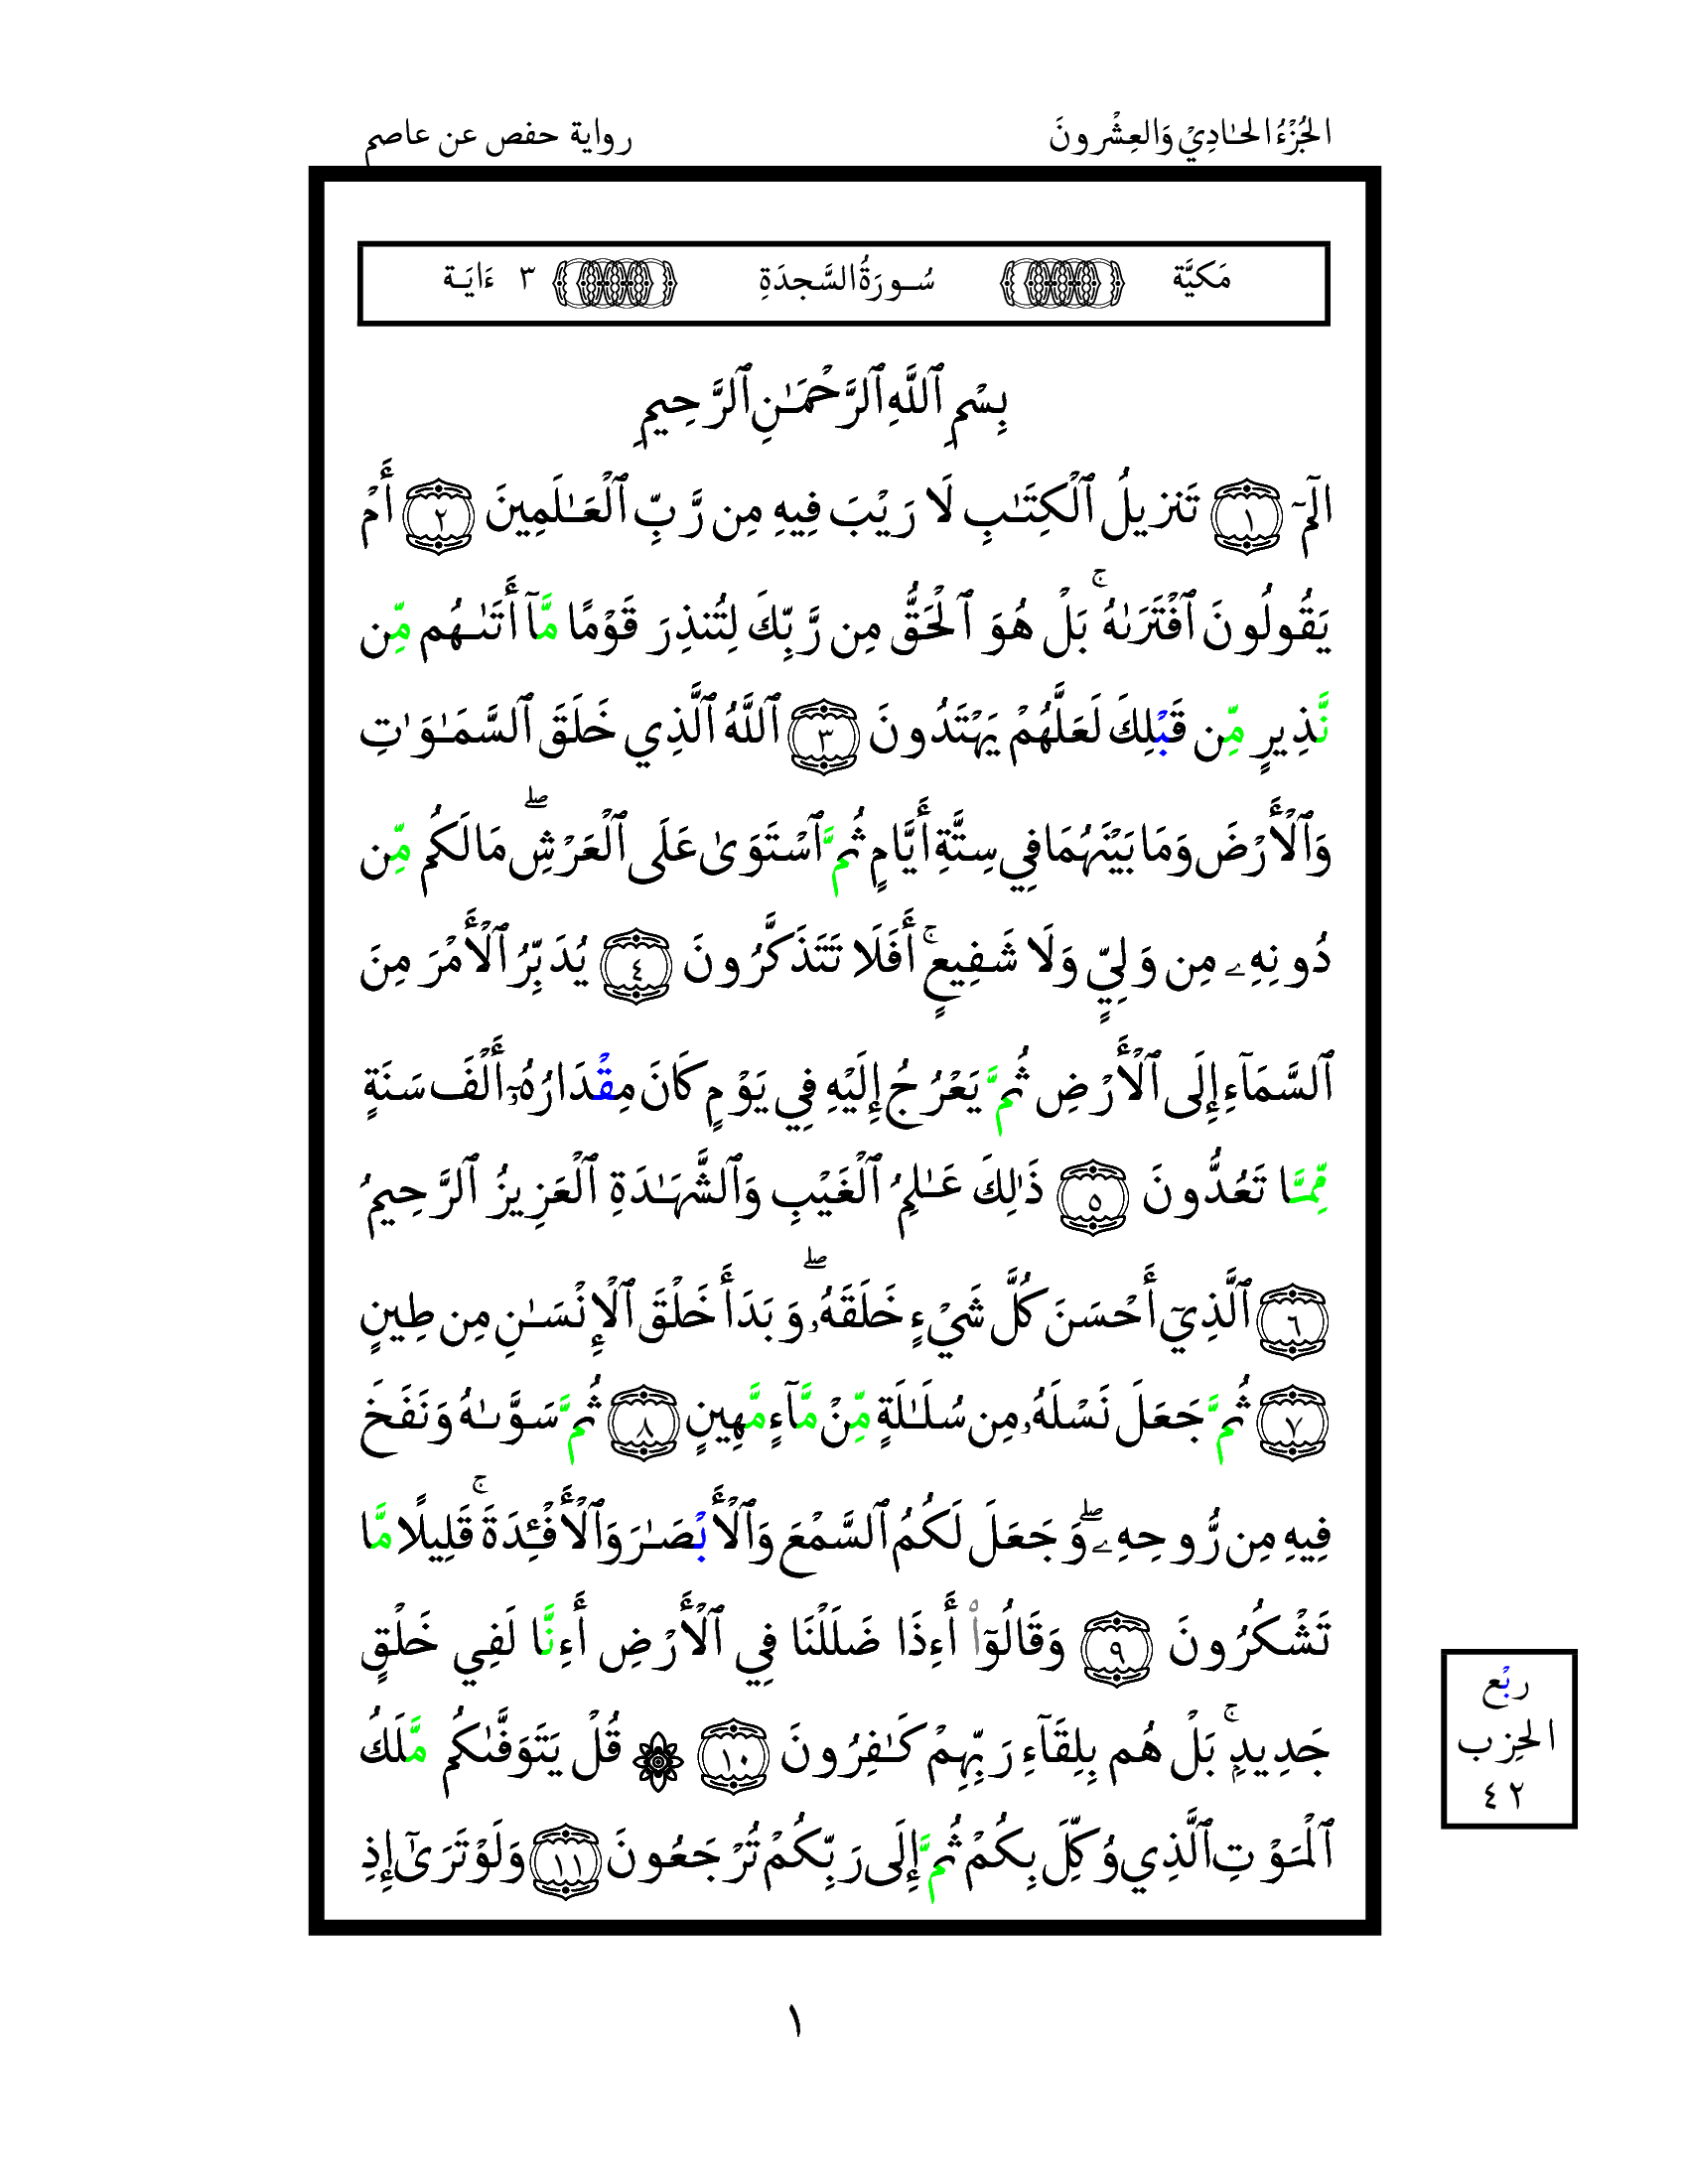
\includegraphics[scale=0.6]{sajdah_1.png}
%}
\end{center}
\end{minipage}

%\begin{minipage}{1\linewidth}
%\begin{center}
%\fbox{
%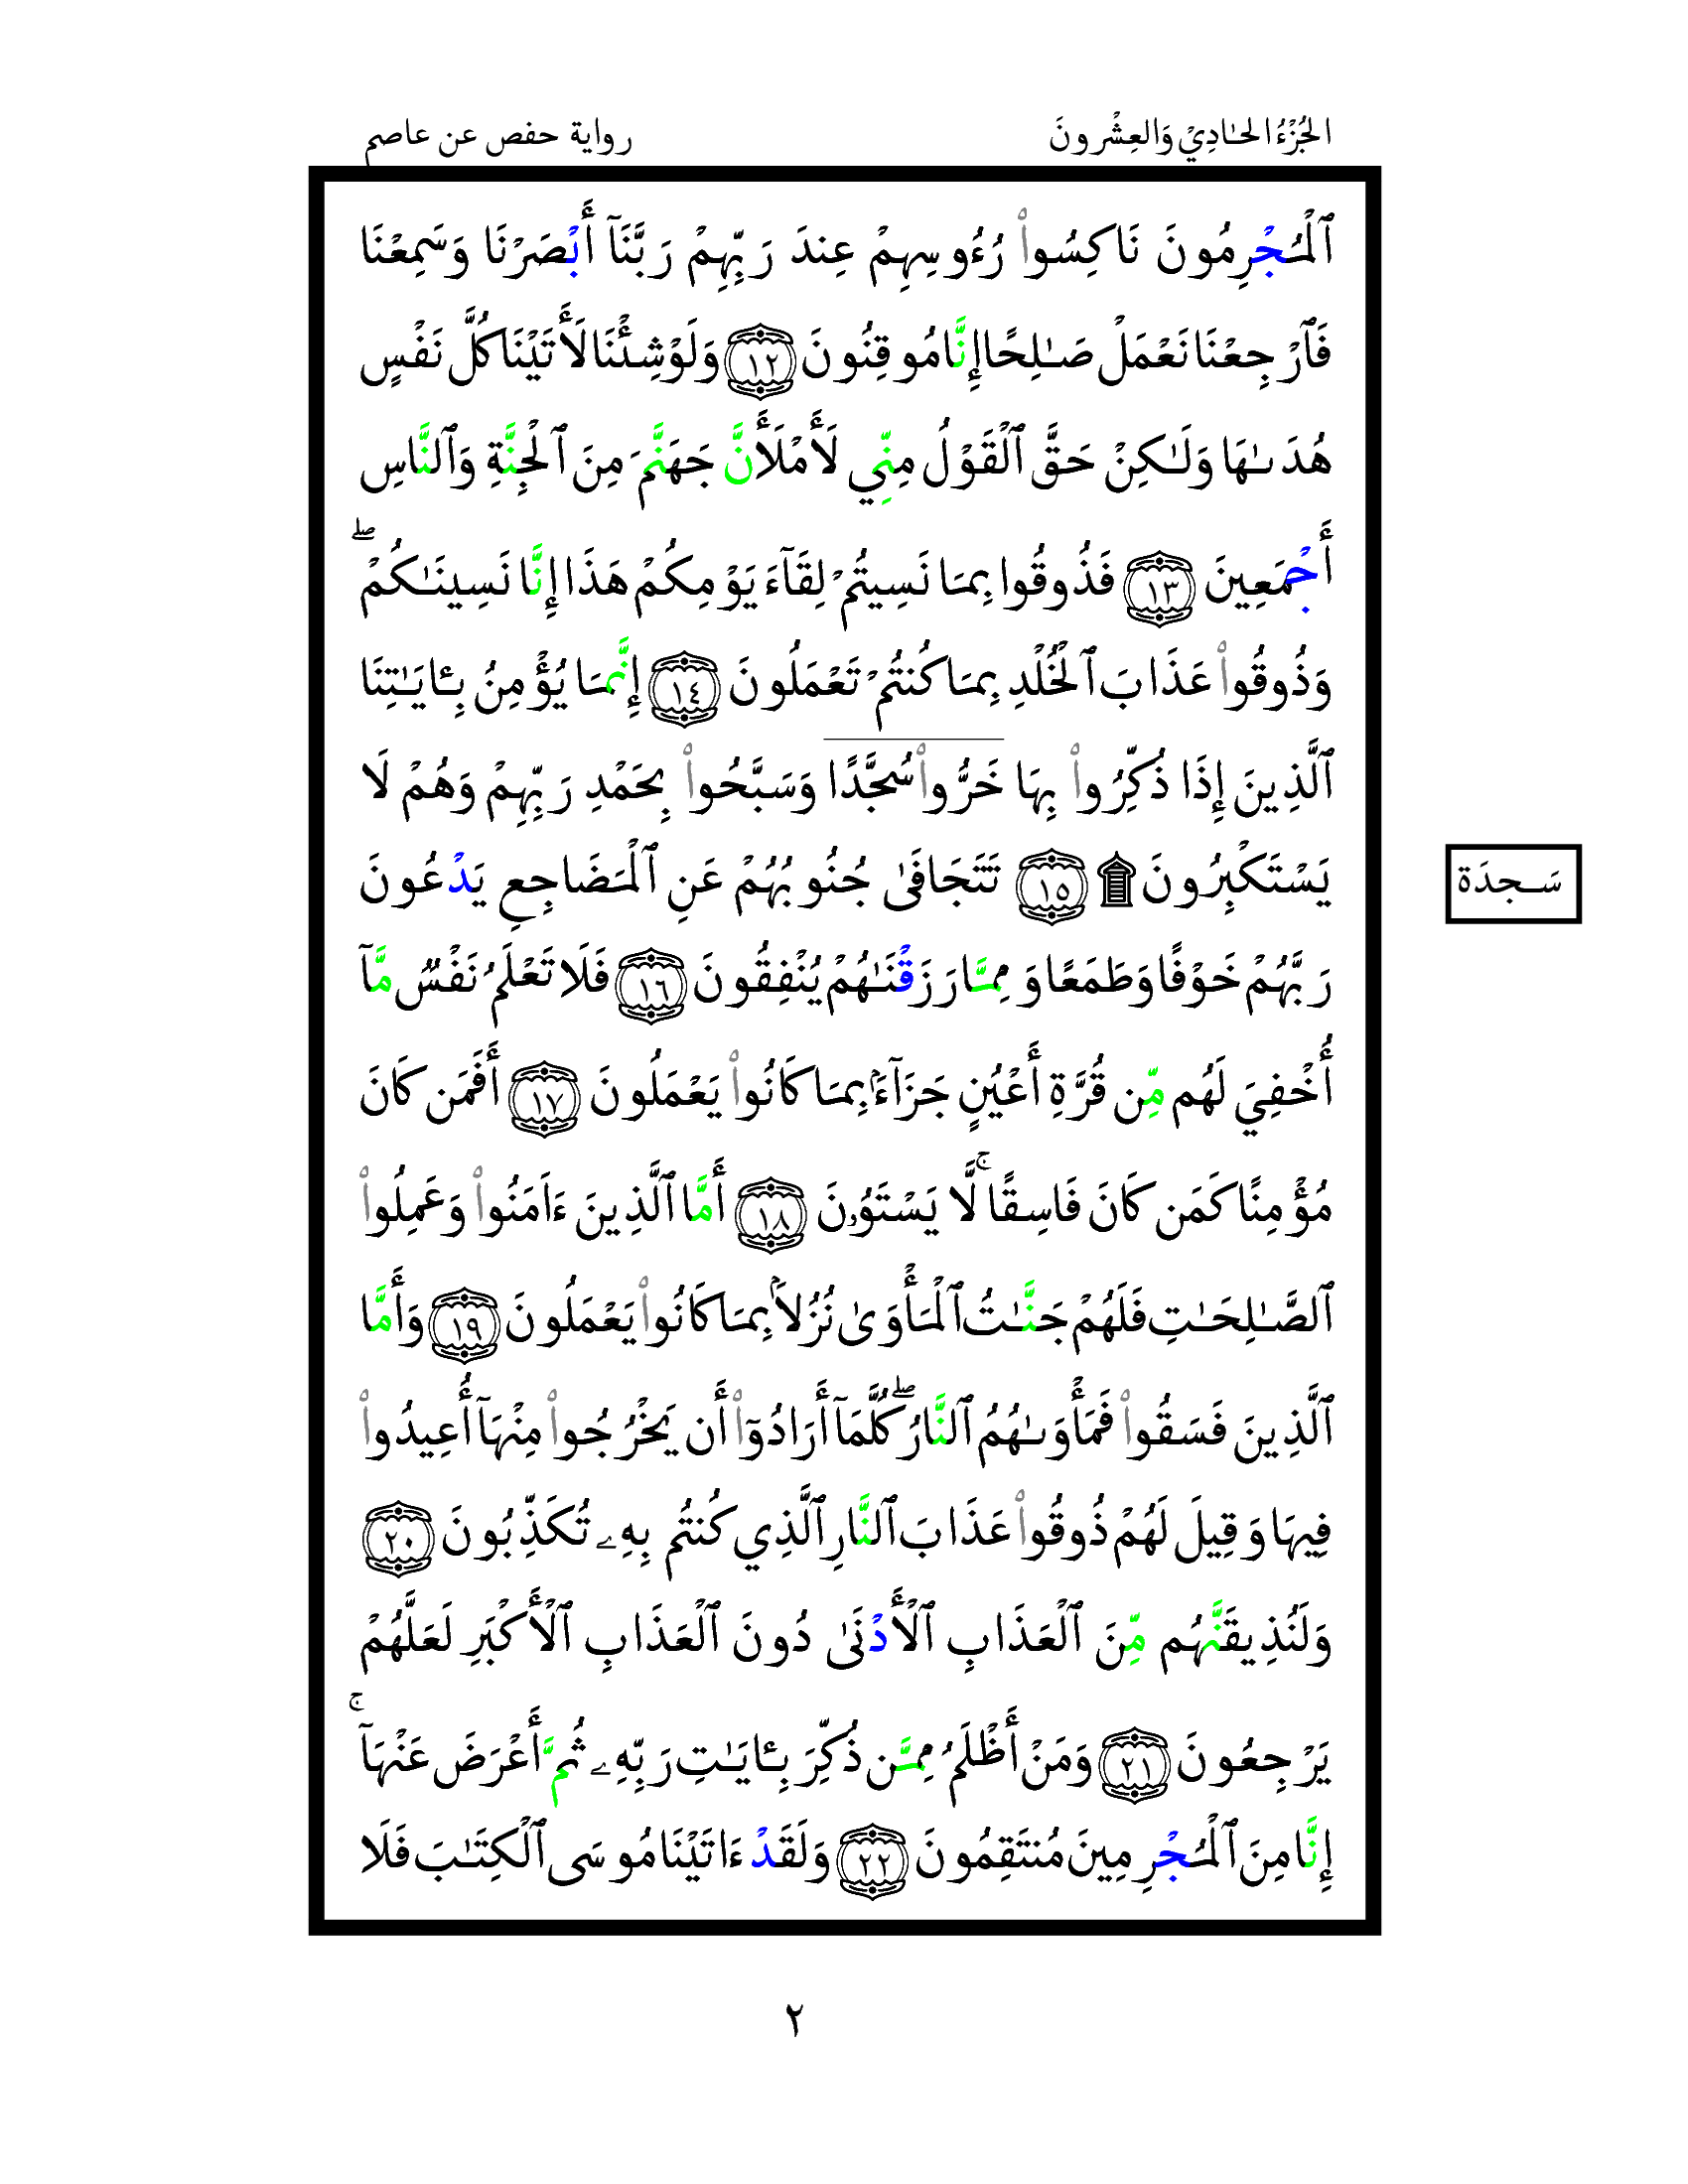
\includegraphics[scale=0.5]{sajdah_2.png}
%}
%\end{center}
%\end{minipage}
%\end{multicols}
%\end{landscape}



\backmatter
\bibliographystyle{is-plain}
\bibliography{bib-buku.bib}

%\chaptername{Ringkasan}
\printnomenclature 
%\chapter{Indeks}
\addcontentsline{toc}{section}{Index} 
\printindex
 \index{mainentry # subentry}
\index{title}

%\chead{\qframe}
/%\rhead{\begin{RLtext}al-salAm `alaykum \end{RLtext}}
%\fancyfoot{}
\setquran

\juz=13
\hizb=25
\fourth=2

\begin{RLtext}
\sura{13}{}{}{43}

\Large
\noindent
\end{RLtext}
%%% Temporarily enlarge this page to push
%% down the bottom margin
\enlargethispage{3\baselineskip}
\thispagestyle{empty}
\pagecolor[HTML]{0E0407}

\begin{center}
\begin{minipage}{.8\textwidth}
\color{Cornsilk}\Large\bfseries
\lipsum[1]

\begin{center}
\huge\bfseries\sffamily\color{lime}`So Calming.'
\end{center}

\lipsum[2]

\end{minipage}
\end{center}

\vspace*{\stretch{1}}

\begin{center}
\colorbox{white}{\EANisbn[SC4]}

\vspace*{\baselineskip}

\textbf{\textcolor{LightGoldenrod!50!Gold}{Malaysian \LaTeX\ User Group \textbullet\ \texttt{http://latex-my.blogspot.com}}}

\textbf{\textcolor{LightGoldenrod}{Cover Illustration by Dusan Bicanski \textbullet\ \texttt{http://www.public-domain-image.com}}}
\end{center}

\end{document}

